\documentclass[10pt,a4paper]{article}
\usepackage[utf8]{inputenc}
\usepackage[czech]{babel}
\usepackage[T1]{fontenc}
\usepackage{amsmath}
\usepackage{amsfonts}
\usepackage{amssymb}
\usepackage{graphicx}
\usepackage{epstopdf}
\usepackage{float}
\usepackage[a4paper,left=3cm,right=3cm,top=2.5cm,bottom=1.5cm]{geometry}
\usepackage[hidelinks]{hyperref}
\usepackage{gensymb}
\addtolength{\footnotesep}{3mm}
\usepackage[bottom]{footmisc}

\title{Sweet Mirage}
\author{Kudlankográl GCHD}
\date{}

\makeatletter
\newcommand{\settitle}{\@maketitle}
\makeatother

\begin{document}

\settitle
\thispagestyle{empty}
\addtocounter{page}{-1}


\begin{figure}[H]
\centering
    \includegraphics[width=0.95\textwidth]{kudlankogral.png}
\end{figure}

\paragraph{}
Název družstva: Kudlankográl GCHD
\paragraph{}
Škola: Gymnázium Christiana Dopplera
\paragraph{}
Adresa: Zborovská 621/45, Praha 5 - Malá Strana, 150 00

\clearpage
\newpage


\author{}
\maketitle
\tableofcontents

\newpage

\section{Zadání}

\subsection{Originální znění}

\paragraph{}
Fata Morgana is the name given to a particular form of mirage. A similar effect can be produced by shining a laser through a fluid with a refractive index gradient. Investigate the phenomenon.\footnote{Zadání úloh | JČMF. JČMF | Jednota českých matematiků a fyziků [online]. Dostupné z: \url{https://www.jcmf.cz/?q=cz/node/1255}}

\subsection{Oficiální překlad}

\paragraph{}
Fata Morgana je název pro konkrétní druh optického klamu. K podobnému jevu může dojít, pokud svítíme laserem skrz tekutinu s gradientem indexu lomu. Prozkoumejte tento jev.\footnote{IYPT 2020 Problems – IYPT.org. IYPT.org – Official IYPT Website [online]. Dostupné z: \url{https://www.iypt.org/index.php/problems/problems-for-the-33rd-iypt-2020/}}


\section{Úvod}
\paragraph{}
Optický jev Fata Morgana můžeme pozorovat na rozsáhlých rovných plochách, jejichž teplota se výrazně liší od teploty okolního vzduchu. To vede k tomu, že se vzduch začne ohřívat či ochlazovat od plochy a nad ní se tak vytvoří vrstvy vzduchu s různou teplotou a tedy i indexy lomu. Paprsky světla vycházející ze vzdáleného objektu procházející takovým prostředím se budou postupně zakřivovat a vzdálený objekt se tak může jevit zrcadlící se ve vzduchu.\footnote{Fata Morgana – Wikipedie. [online]. Dostupné z: \url{https://cs.wikipedia.org/wiki/Fata_morg\%C3\%A1na}}

\begin{figure}[H]
\centering
    \includegraphics[width=0.8\textwidth]{fatamor.png}
    \label{fig:uvod}
    \caption[Caption for LOF]{Zakřivení paprsku při průchodu prostředím s gradientním indexem lomu.\protect\footnotemark}
\end{figure}

\footnotetext{Pavement Mirage Diagram.svg - Wikimedia Commons. [online]. Dostupné z: \url{https://commons.wikimedia.org/wiki/File:Pavement_Mirage_Diagram.svg}}

\paragraph{}
Podobný efekt můžeme pozorovat v roztoku vody a cukru, kde cukr klesne na dno a difúzí se začne promíchávat s vodou. Tím vzniknou vrstvy roztoku o různých indexech lomu schopné zakřivovat světelné paprsky.

\section{Abstrakt}
\paragraph{}
V rámci této úlohy jsme se zabývali schopností roztoku s gradientním indexem lomu stáčet rovinu polarizace a zaostřovat či rozostřovat paprsek.
Byl vytvořen postup pro získání rozložení indexů lomu v prostředí z fotky paprsku, který jím prochází. Pomocí něj jsme simulovali trajektorii paprsku a také stáčení roviny polarizace, zaostřování a rozostřování paprsku.

\newpage

\section{Popis Experimentu}
\paragraph{}
Použili jsme akvárium s rozměry podstavy 5x65cm a výškou 15cm. Do něj jsme nalili vodu a poté opatrně přidali roztok s cukrem. Do roztoku jsme také přidali fluorescenční barvivo pro zvýraznění trajektorie laseru.

\paragraph{}
Přes boční stěnu akvária bylo možné pozorovat velmi navýraznou Fata Morganu.


\begin{figure}[H]
\centering
    \includegraphics[width=\textwidth]{ukazkaAkvarko.jpg}
    \label{fig:uvod}
    \caption{Ukázka experimentu}
\end{figure}

\newpage

\section{Popis výpočtu}

\subsection{Rozložení indexů lomu v prostředí}

\paragraph{}
Trajektorii paprsku z fotografie získáme jednodušše, z každého sloupce vybereme nejsvětlejší pixel, čímž získáme všechny pixely nacházející se na trajektorii paprsku. Tyto body ještě klouzavým průměrem vyhladíme.


\begin{figure}[H]
\centering
    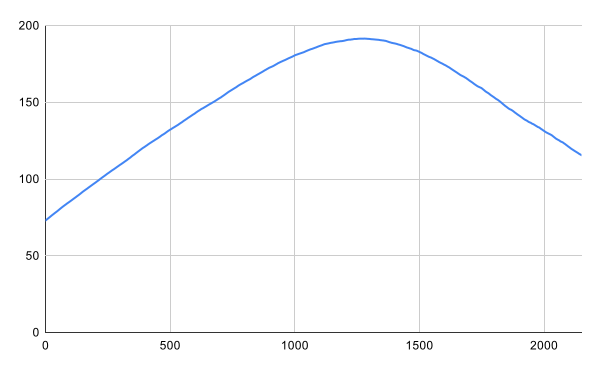
\includegraphics[width=0.9\textwidth]{chart.png}
    \caption{Vyhlazená trajektorie z úvodní fotografie}
    \label{fig:chart1}
\end{figure}

\paragraph{}
Indexy lomů na jednotlivých vrstvách ze získaných bodů můžeme vyjádřit iteračně pomocí Snellova zákona.\footnote{Snellův zákon – Wikipedie. [online]. Dostupné z: \url{https://cs.wikipedia.org/wiki/Snell\%C5\%AFv_z\%C3\%A1kon}}


\begin{equation*}
  \alpha_{i+1} = arctan\left ( \left |  \frac{x_{i+1} - x_{i}}{y_{i+1} - y_{i}} \right | \right )
\end{equation*}

\begin{equation*}
  n_{i+1}=\frac{n_{i} \cdot  sin(\alpha _{i})}{sin(\alpha _{i+1})}
\end{equation*}

Kde $x_{i}, y_{i}$ jsou souřadnice bodů po pořadě od nejnižího po nejvyšší,
$\alpha_{i}$ je úhel dopadu na vrstvu ve výšce bodu $i$ a $n_{i}$ je index lomu ve výšce bodu $i$


\begin{figure}[H]
\centering
    \includegraphics[width=0.9\textwidth]{n1-prohozene.png}
    \caption{Vypočtené rozložení indexů lomu z vyhlazené trajektorie}
    \label{fig:chart1}
\end{figure}

\paragraph{}
Na obrázku 4 si můžeme všimnout zvlnění křivky závislosti indexu lomu na výšce, to je pravděpodobně způsobeno rozvýřením roztoku jeho neustálým promícháváním difúzí.

\paragraph{}
Zpracováním několika fotografií jsme zjistili, že rozdíly v indexech lomů mezi spodní a vrchní hladinou jsou v řádech tisícin až setin. Tyto rozdíly zdaleka nedosahují přesnosti měření s refraktometrem, které jsme také provedli. Na simulaci trajektorií paprsků nám ale stačí znát poměry mezi indexy na sousedních hladinách a ty jsme schopní získat.


\subsection{Ostření laseru}

\paragraph{}
K zaostření a rozostření laseru dochází kvůli posunutí jednotlivých paprsků v laseru na y-ové ose, to způsobí, že paprsky vstpují do vrstev s různým indexem lomu a než spodní paprsek doputuje ke vstupní vrstvě horního paprsku, tak se již pohybuje pod jiným úhlem a tedy i po jiné trajektorii.
Tento jev můžeme předpovídat pomocí simulování trajektorie dvou paprsků posunutých vůči sobě v y-ové ose, které vstupují do prostředí pod stejným úhlem měřeným od svislého směru. Budou-li na konci vůči sobě blíže než-li na začátku došlo k zaostření, jinak k rozostření.


\begin{figure}[H]
\centering
    \includegraphics[width=\textwidth]{simtraj.png}
    \caption{Simulovaná trajektorie paprsků vzdálených od sebe 8 pixelů vstupující do prostředí našeho roztoku cukru pod úhlem 1,513 radiánů. Můžeme pozorovat efekt zaostření.}
    \label{fig:chart1}
\end{figure}

\subsection{Stáčení roviny polarizace}

\paragraph{}
Dále jsme se pomocí Fresnelových rovnic\footnote{Fresnelovy rovnice – Wikipedie. [online]. Dostupné z: \url{https://cs.wikipedia.org/wiki/Fresnelovy_rovnice}}
 pokusili simulovat stočení roviny polarizace paprsku při průchodu prostředím. Simulováním na základě několika různých naměřených rozložení indexů lomu v akváriu jsme zjistili, že vliv Fresnelových rovnic na stočení roviny polarizace je zanedbatelný, rozdíl většinou je až na pátém desetinném místě. Ovšem při experimentu s cukerným roztokem bude mít na stočení roviny polarizace velký vliv měrná stáčivost sacharózy\footnote{Specific rotation - Wikipedia. [online]. Dostupné z: \url{https://en.wikipedia.org/wiki/Specific_rotation}}, tu jsme v našem roztoku pomocí polarimetru naměřili na 9\degree{}/dm
 .
 Vliv Fresnelových rovnic je tedy, alespoň v našem roztoku, zcela neměřitelný, a tak jsme se stáčením roviny polarizace již dále nezabývali.

\newpage

\section{Srovnání simulace ostření paprsku s experimentem}

\subsection{Získání rozložení indexů lomu}
\paragraph{}
Pro experiment jsme pořídili celkem tři fotografie ze stejné pozice a úhlu. Na fotografiích je zachycen průchod paprsku roztokem cukru. 
\paragraph{}
Na jedné fotografii laser vstupuje do akvária níže a vychází výše než-li na ostatních dvou fotografiích, je tedy vhodný pro výpočet rozložení indexů lomu v akváriu.
\paragraph{}
Na dalších dvou fotografiích je laserový paprsek rozdělen milimetrovým proužkem na dva, čímž se zvýrazní fokusovací efekt při průchodu prostředím.

\begin{figure}[H]
\centering
    \includegraphics[width=0.8\textwidth]{image9.jpg}
    \caption{Fotografie pro určení rozložení indexů lomu}
    \label{fig:chart1}
\end{figure}

\paragraph{}
Nejprve získáme trajektorii paprsku

\begin{figure}[H]
\centering
    \includegraphics[width=\textwidth]{image4.png}
    \caption{Trajektorie paprsku}
    \label{fig:chart1}
\end{figure}

\paragraph{}
Z níž vypočteme rozložení indexů lomu

\begin{figure}[H]
\centering
    \includegraphics[width=0.9\textwidth]{n2-prohozeny.png}
    \caption{Rozložení indexů lomu}
    \label{fig:chart1}
\end{figure}

\subsection{Simulování situace v první fotografii}

\begin{figure}[H]
\centering
    \includegraphics[width=0.9\textwidth]{image8.jpg}
    \caption{Oříznutá fotografie}
    \label{fig:chart1}
\end{figure}

\begin{figure}[H]
\centering
    \includegraphics[width=0.9\textwidth]{rozbihavy-protazeny.jpg}
    \caption{Roztažený paprsek na fotografii}
    \label{fig:chart1}
\end{figure}

\paragraph{}
Rozdíl výšky paprsků jsme vypočetli jako 8 pixelů. Jako počátek jsme z fotky určili 1988. pixel ze spoda a úhel při vstupu 1,512 radiánů.
Můžeme zde pozorovat rozbíhání paprsků, tedy rozostřování. Což je také výsledkem naší simulace.

\begin{figure}[H]
\centering
    \includegraphics[width=\textwidth]{rozbihavy.png}
    \caption{Předpověď simulace}
    \label{fig:chart1}
\end{figure}



\subsection{Simulování situace v druhé fotografii}

\begin{figure}[H]
\centering
    \includegraphics[width=0.9\textwidth]{image7.jpg}
    \caption{Oříznutá fotografie}
    \label{fig:chart1}
\end{figure}

\begin{figure}[H]
\centering
    \includegraphics[width=0.9\textwidth]{sbihavy-protazeny.jpg}
    \caption{Roztažený paprsek na fotografii}
    \label{fig:chart1}
\end{figure}

\paragraph{}
Zde byl použit stejný milimetrový proužek na rozdělení paprsku a také paprsek vstupoval do prostředí ve stejné výšce jako předtím. Úhel vstupu paprsku byl z fotky změřen na 1,526 radiánů.
Můžeme zde pozorovat protnutí obou paprsků a následné rozbíhání, což také vychází ze simulace.


\begin{figure}[H]
\centering
    \includegraphics[width=\textwidth]{sbihavygraf.png}
    \caption{Předpověď simulace}
    \label{fig:chart1}
\end{figure}


\section{Závěr}

\paragraph{}
Vytvořili jsme numerické simulace pro získání rozložení indexů lomu z fotografie, trajektorie paprsku v prostředí a stáčení roviny polarizace vlivem Fresnelových zákonů. 
\paragraph{}
    Zjistili jsme, že rozdíli indexů lomu ve vrstvách našeho roztoku jsou obvyklými metodami neměřitelné, stejně tak je tomu se stočením roviny polarizace vlivem Fresnelových rovnic. Povedlo se nám ovšem úspěšně pomocí simulace trajektorie paprsku předpovědět jeho zaostření a rozostření při průchodu prostředím.

\end{document}